\documentclass[final]{article}

% if you need to pass options to natbib, use, e.g.:
% \PassOptionsToPackage{numbers, compress}{natbib}
% before loading nips_2017
%
% to avoid loading the natbib package, add option nonatbib:
% \usepackage[nonatbib]{nips_2017}

\usepackage{nips_2017}
\usepackage{graphicx,url}
\usepackage{amsmath}
%\usepackage{algorithm}
%\usepackage[noend]{algpseudocode}
\usepackage{balance}
\usepackage{gensymb}
\usepackage{multirow}
\usepackage{hhline}
\usepackage{array}
\usepackage[font=small,labelfont=bf]{caption}
\usepackage{dblfloatfix}
\usepackage{gensymb}
\usepackage{movie15}
% to compile a camera-ready version, add the [final] option, e.g.:
% \usepackage[final]{nips_2017}

\usepackage[utf8]{inputenc} % allow utf-8 input
\usepackage[T1]{fontenc}    % use 8-bit T1 fonts
\usepackage{hyperref}       % hyperlinks
\hypersetup{
    colorlinks=true,
    linkcolor=blue,
    filecolor=magenta,      
    urlcolor=blue,
}
\usepackage{url}            % simple URL typesetting
\usepackage{booktabs}       % professional-quality tables
\usepackage{amsfonts}       % blackboard math symbols
\usepackage{nicefrac}       % compact symbols for 1/2, etc.
\usepackage{microtype}      % microtypography

\title{Assignment 1: PID and Model Predictive Control}
% The \author macro works with any number of authors. There are two
% commands used to separate the names and addresses of multiple
% authors: \And and \AND.
%
% Using \And between authors leaves it to LaTeX to determine where to
% break the lines. Using \AND forces a line break at that point. So,
% if LaTeX puts 3 of 4 authors names on the first line, and the last
% on the second line, try using \AND instead of \And before the third
% author name.
%\author{
%  Patrick Lancaster\\
%  Paul G. Allen School of Computer Science and Engineering\\
%  University of Washington\\
%  Seattle WA, 98195 \\
%  \texttt{planc509@cs.washington.edu} \\
  %% examples of more authors
  %% \And
  %% Coauthor \\
  %% Affiliation \\
  %% Address \\
  %% \texttt{email} \\
  %% \AND
  %% Coauthor \\
  %% Affiliation \\
  %% Address \\
  %% \texttt{email} \\
  %% \And
  %% Coauthor \\
  %% Affiliation \\
  %% Address \\
  %% \texttt{email} \\
  %% \And
  %% Coauthor \\
  %% Affiliation \\
  %% Address \\
  %% \texttt{email} \\
%}
\begin{document}
%\nipsfinal
\maketitle
In this assignment, you will implement two methods for controlling the RACECAR. First, you will design a PID controller to control the robot's steering angle as it tries to follow a line (which is represented by a plan consisting of a sequence of poses). Second, you will use model predictive control to allow the robot to wander around without crashing while simultaneously minimizing its steering angle control effort. Note that in this assignment, many of the implementation details will be left up to you. We encourage you to try out different implementations in order to get the best results. The provided \href{https://gitlab.cs.washington.edu/uw_racecar/course_materials/lab1}{skeleton code} does have \textit{suggestions} for \textit{some} of these details.

This assignment can be done as a group. Only one member of the group needs to submit it to the Canvas dropbox. All group members' names should be on the document containing answers to the assignment's questions.

\section{Getting Started}
Here is some prerequisite information for this assignment:

\begin{enumerate}
\item Please git pull the \textit{racecar\_base\_public} repository
\item Before running the updated simulation, install networkx: \textit{sudo easy\_install networkx}
\item Once you run teleop.launch, the simulation will start generating a graph file for the current map. This will take a few minutes to complete. However, the simulation will save the graph file so that it only ever has to be done once per map.
\item While running teleop.launch, you can use the \texttt{2D Pose Estimate} button in the upper ribbon to specify the pose of the robot. You can also use the \texttt{2D Nav Goal} in the upper ribbon to specify a goal pose for the robot. If you have done both of these, the simulation will begin computing a plan from the robot's current pose to the goal pose. This may take a while depending on the map (you can view its progress by looking at the terminal where you launched teleop.launch), but the result can be viewed under the PoseArray topic \textit{/planner\_node/car\_plan}
\item You can change the map that is used by the simulation by editing the 'map' argument of \texttt{racecar\_base\_public/racecar/launch/includes/common/map\_server.launch}. It can reference any of the .yaml files found inside of \texttt{racecar\_base\_public/racecar/maps}
\item Skeleton code for this assignment is available \href{https://gitlab.cs.washington.edu/uw_racecar/course_materials/lab1}{here}.
\end{enumerate}

\section{Line Following with PID Control}
In this section, you will use PID control to steer your robot along a provided plan to reach a goal  pose. It is up to you to define the exact error metric (within reason), as well as the values of the parameters that affect the control policy. Note that only the steering angle is being varied - the robot's forward velocity should be constant.

\subsection{In Simulation}
Write a script in \textbf{line\_follower.py} that does the following:

\begin{enumerate}
\item Receives a plan generated by the simulation
\item Subscribes to the current pose of the robot
\item For each received pose
 \begin{enumerate}
 \item Determine which pose in the plan the robot should navigate towards. This pose will be referred to as the target pose.
 \item Compute the error between the target pose and the robot.
 \item Store this error so that it can be used in future calculations (particularly for computing the integral and derivative error)
 \item Compute the steering angle $\delta$ as \\
 
  \centerline{$\delta = k_p*e_t + k_i* \int e_t dt + k_d* \frac{de_t}{dt}$}
 
 \item Execute the computed steering angle. 
 \end{enumerate}
\end{enumerate}

Also, fill in the launch file \textbf{line\_follower.launch} in order to launch your node. Use this launch file to vary the parameters of your system.

Test your system by playing back the provided bag file (lab1/bags/line\_follower.bag) when using the 'small\_basement' map. The bag file will automatically specify the initial and goal pose - i.e. you don't need to manually specify the initial pose and goal pose in rviz. Choose 3 different sets of PID parameters, where each set specifies a controller that causes the robot to successfully navigate from the start to the goal. Measure the performance of these controllers by recording the error at each iteration of the pose callback. Plot all three data series on a single figure where the y axis is the error and the x axis is the iteration index.

Hint: Try your script out on the simple map first so that it doesn't take a long time to compute a plan. Or, you could have the simulation generate a plan and then create a bag of the plan, which you could then replay whenever you want to test your code.

For more details, see the provided skeleton code.

\section{Wandering Around with MPC}

In this section, you will use the kinematic car model to simulate possible trajectories for your robot to follow. Based on received laser scans, your robot will execute a steering angle control that avoids obstacles while minimizing the steering angle control effort. Note that only the steering angle is being varied - the robot's forward velocity should be constant.

\subsection{In Simulation}

Write a script in \textbf{laser\_wanderer.py} that does the following:
\begin{enumerate}
\item Rolls out n trajectories and caches them
\item Vizualizes the final pose of each trajectory as the car moves around in the world, such as in Fig. \ref{fig:rollouts} below. This will require subscribing to the pose of the robot.

\begin{figure*}[h]
\centering
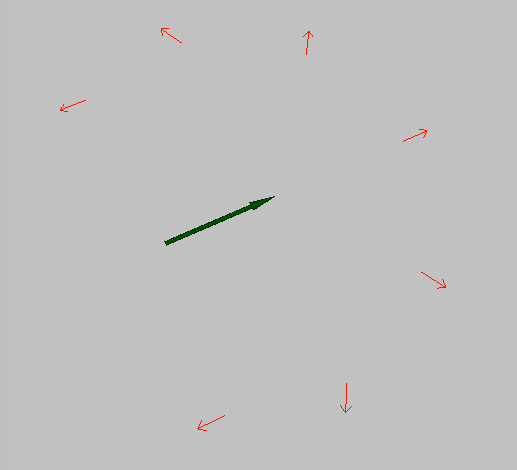
\includegraphics[width=0.45\linewidth]{figs/rollouts.png}
\caption{The robot in green and the final pose of each trajectory in red}
\label{fig:rollouts}
\end{figure*}
 
\item Subscribes to the robot's laser scans
\item Whenever a laser scan is received, spend a fixed amount of time computing the trajectory costs as illustrated in Fig. \ref{fig:any_time}
	\begin{enumerate}
	\item Compute the cost of the first step of each trajectory.
	\item If there is remaining computation time, compute the cost of the second step of each trajectory and add them to the cost of the first trajectory steps.
	\item Continue this process until the allowed amount of computation time has expired.
	\begin{figure*}[h]
	\centering
	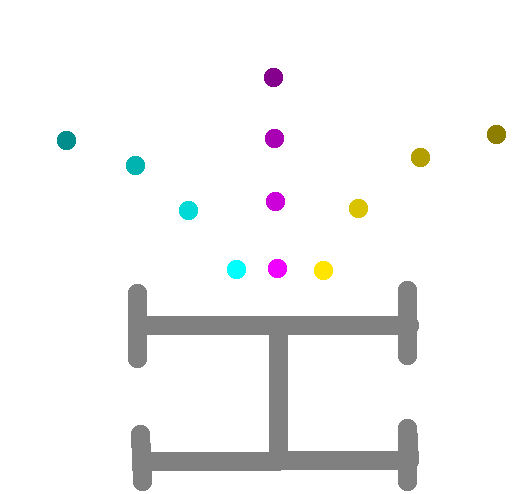
\includegraphics[width=0.4\linewidth]{figs/any_time.png}
	\caption{Three different trajectories. Earlier steps of the trajectories are drawn in lighter shades, while later steps of the trajectories are drawn in darker shades. Under the specified any-time algorithm scheme, the costs of the lighter shaded poses are first computed, and the cost of the darker shaded poses are only computed if there is computation time remaining.}
	\label{fig:any_time}
	\end{figure*}
	\end{enumerate}
	\item Chooses the steering angle that corresponds to the least costly trajectory and executes it
\end{enumerate}

Given a pose in a trajectory to compute the cost for, initialize the cost as the magnitude of the steering angle that corresponds to that trajectory. Then consider the line that emanates from the robot to the pose. Calculate the angle $\theta$ between this line and the x-axis of the robot, as shown in Fig. \ref{fig:scan_cost}. Then find the laser ray that corresponds to $\theta$. If the laser ray measurement is closer than the pose, then a heavy penalty should be added. If the laser ray measurement is further away than the pose, then the pose does not incur additional cost. 

\begin{figure*}[h]
\centering
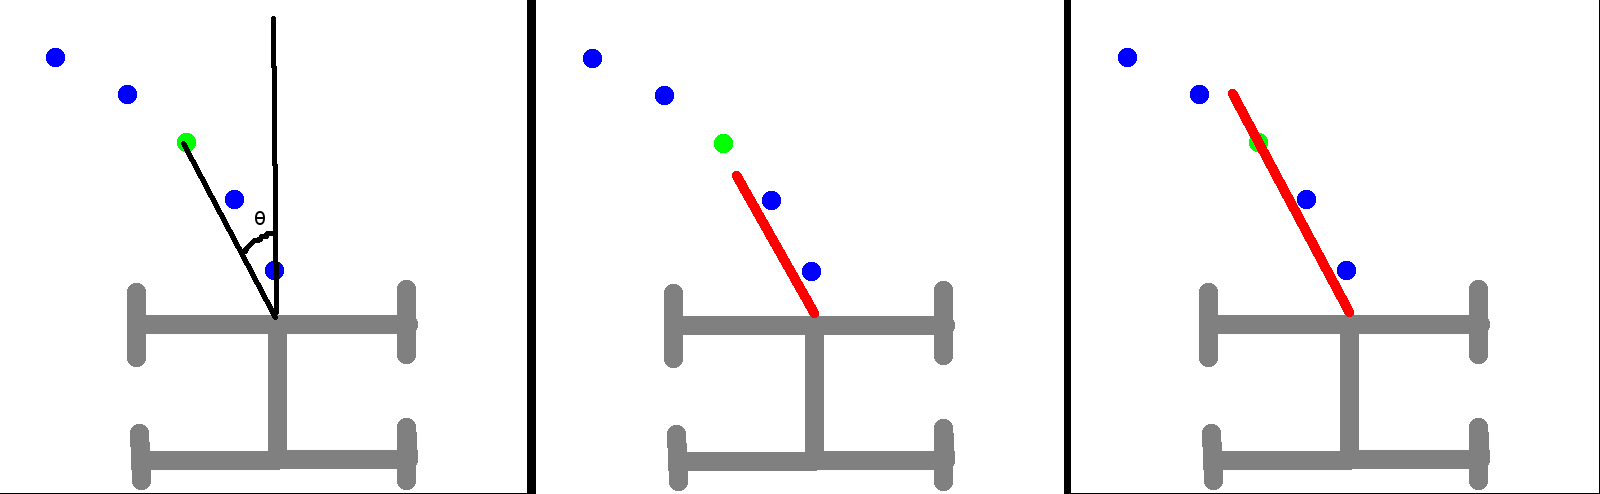
\includegraphics[width=\linewidth]{figs/scan_cost.png}
\caption{Left: The cost of the green pose is being computed. Middle: The corresponding laser ray in red is closer than the pose, so the pose receives a large penalty. Right: The corresponding laser ray is farther than the pose, so no additional penalty is incurred. }
\label{fig:scan_cost}
\end{figure*}


Hint: To check that you are calculating the costs correctly, initialize your robot in different poses and print out the costs of each trajectory (but don't publish any controls so that your robot doesn't actually move). Check if these costs make sense.

Finally, implement the \textbf{laser\_wanderer.launch} file to launch your node.

Test your system by playing back the provided bag file (lab1/bags/laser\_wanderer.bag) when using the 'no-end-floor4\_corridor' map. The bag file will automatically specify the initial pose - i.e. you don't need to manually specify the initial pose in rviz. 

For more details, see the provided skeleton code.

\subsection{On Robot}

The robot is no longer a point in space - it now has width! Modify your algorithm to account for this. 

\newpage

\section{Assignment Submission}

Submit the following:

\subsection{Line Following with PID Control}
\begin{enumerate}
\item Answer: What exactly was your error metric? How exactly did you choose which point the robot should navigate towards?
\item Answer: What are the 3 sets of PID parameters that you choose? Which set of PID parameters performed best? Why do you think this is the case?
\item Answer: What is missing that is stopping us from implementing this on the real robot?
\item The error plot described at the end of Section 2.1
\item A video of your best PID controller following the path generated by the provided bag file
\item Your line\_follower.py script and line\_follower.launch launch file
\end{enumerate}

\subsection{Wandering Around with MPC}
\begin{enumerate}
\item Answer: Describe the parameter values that you chose (e.g. T, delta\_incr, etc.). Describe any other design choices that you made.
\item A video of your robot continuously wandering around the no-end-floor4\_corridor map for at least one minute when initialized by the provided bag. Make sure the robot's laser scan and the vizualization you implemented are visible.
\item Your laser\_wanderer.py script and laser\_wanderer.launch launch file
\end{enumerate}

In addition, if you are working with the real robot, answer the following: \\
Describe the changes you made when transferring from the simulated robot to the real robot, if any.

You will also demo your robot wandering around the EE basement. The requirement will be that your robot should continuously wander around without crashing for at least 30 seconds. 

\end{document}

